\chapter{Il progetto \ProjectTitle}
\thispagestyle{stdPage}
% Grid with 1 row and 3 columns for images inside the folder slides
\begin{figure}[H]
    \begin{subfigure}{0.33\textwidth}
        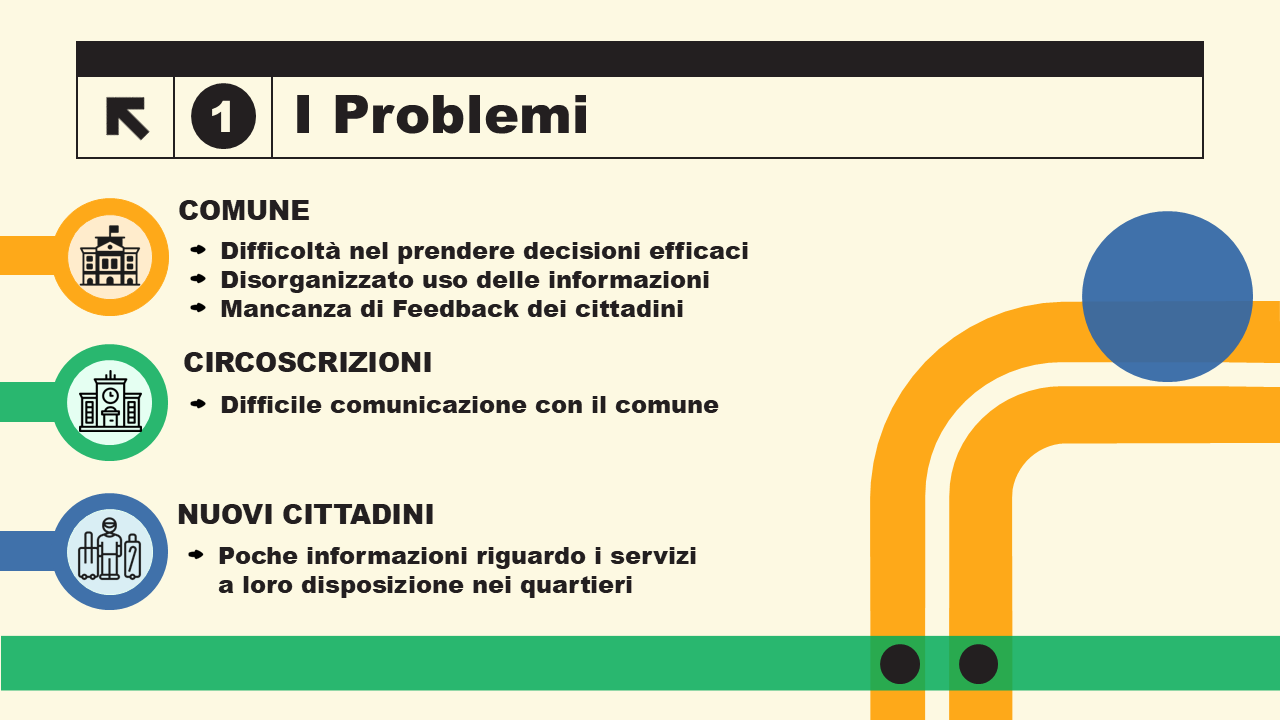
\includegraphics[width=\textwidth]{slides/Diapositiva2.PNG}
        \caption{I problemi}
    \end{subfigure}
    \begin{subfigure}{0.33\textwidth}
        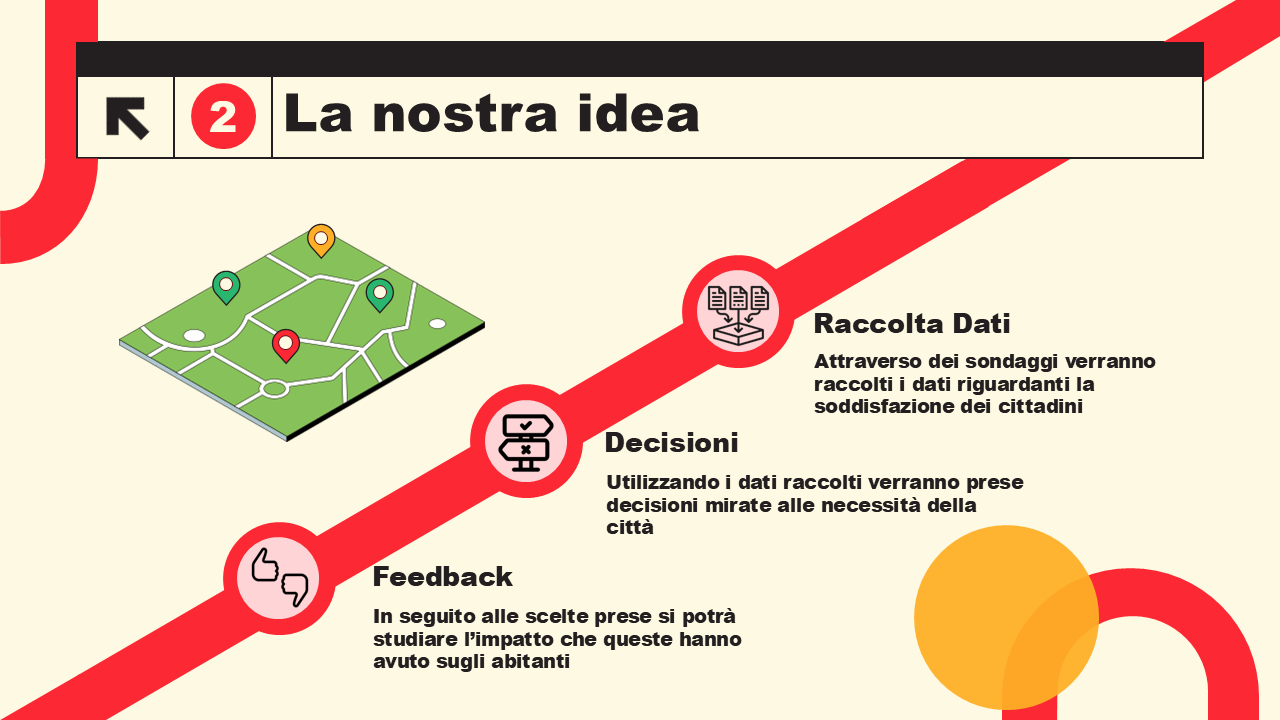
\includegraphics[width=\textwidth]{slides/Diapositiva3.PNG}
        \caption{La soluzione}
    \end{subfigure}
    \begin{subfigure}{0.33\textwidth}
        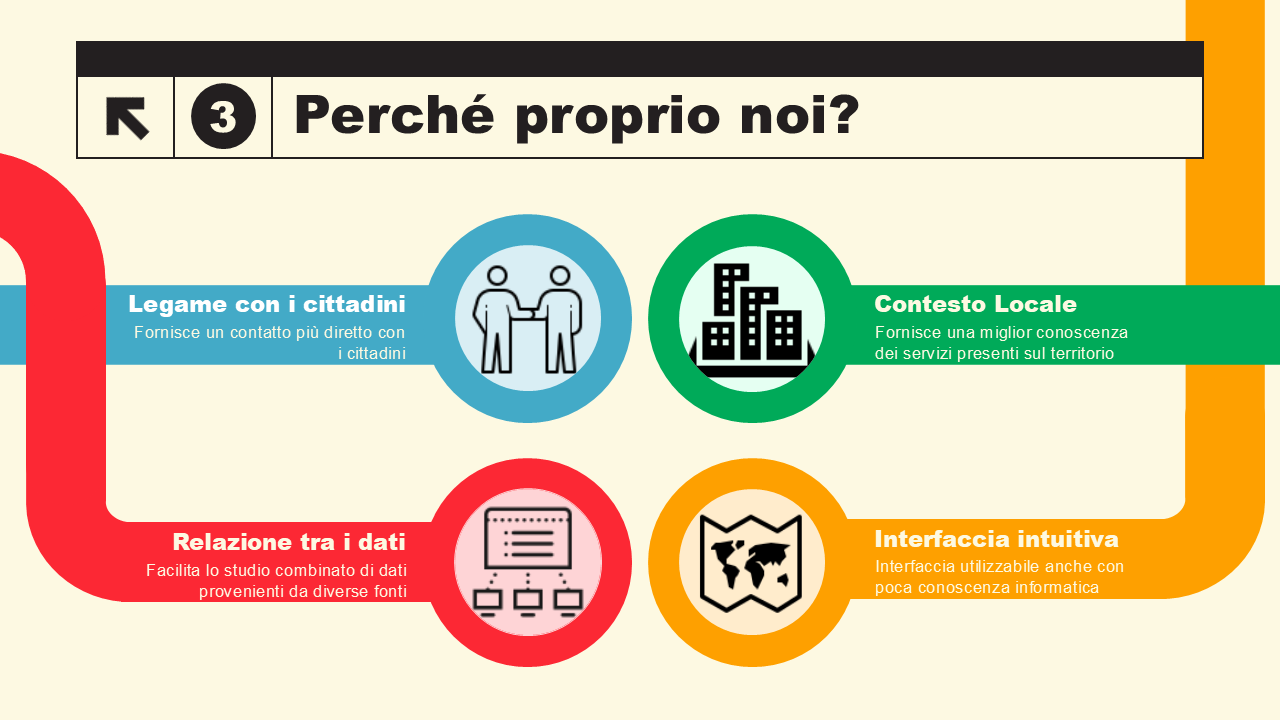
\includegraphics[width=\textwidth]{slides/Diapositiva4.PNG}
        \caption{I vantaggi}
    \end{subfigure}
\end{figure}

\section{I problemi}
    Il progetto mira a risolvere due problemi. Il primo problema riguarda una difficoltà che colpisce l'amministrazione del Comune di Trento, più precisamente la difficoltà stante nel processo di prendere decisioni amministrative efficaci per la città, infatti non raramente accade che una decisione fatta dal Comune non porti al risultato atteso o desiderato. Questo problema nasce dal fatto che, attualmente, il personale del comune non dispone di un modo adeguatamente chiaro, semplice, e organizzato di studiare la mole di dati rilevanti alla situazione della città. Inoltre, i modi esistenti in cui il Comune ottiene un riscontro dai cittadini veri e propri sulla loro soddisfazione con la città sono insufficienti o inaffidabili, rendendo difficile comprendere l'impatto delle decisioni prese in passato. 
    
    Il secondo problema riguarda gli abitanti che si sono trasferiti, sono ancora nel processo di trasferirsi, o sono interessati a trasferirsi, a Trento. Questi nuovi cittadini spesso sono ignari dei servizi a loro disponibili nell'area in cui si trovano, e dunque non sono in grado di usufruirne. Inoltre, non hanno una visione chiara della situazione della città, e dunque non sono in grado di valutare se un particolare quartiere o zona della città sia adatta alle loro esigenze. Questo problema è aggravato dal fatto che i dati sulla città sono spesso dispersi in vari siti web e documenti, e non sono presentati in modo chiaro e comprensibile.

\section{La soluzione}
    L'obbiettivo del progetto è realizzare un'applicazione web che permetterà sia ai cittadini che al personale del Comune di visualizzare in modo intuitivo e comprensibile i dati sui servizi presenti nella città, la grande parte di questi dati è gia stata raccolta, hanno solo bisogno di essere mostrati agli utenti. Oltre a queste informazioni l'applicazione mostrerà anche l'andamento nel tempo del grado di felicità, espresso in percentuale, della popolazione della città e dei singoli quartieri. I dati sulla felicità potranno essere raccolti da tipi di fonti diversi.

    L'applicazione sarà accessibile tramite browser, qualunque utente sarà in grado di vedere dei dati generali sulla città. Il personale del Comune, una volta autenticatosi, avrà accesso ad ulteriori funzionalità per aggiungere, modificare, analizzare, e rimuovere dati dal sistema. Il software sarà conforme alle normative vigenti riguardo la protezione delle informazioni e delle credenziali di accesso degli utenti del Comune.


\section{I vantaggi - sia per il Comune che per i Cittadini}
    \begin{itemize}
        \item \textbf{Legame con i Cittadini: la possibilità di visualizzare in modo semplice la felicità attuale e passata dei residenti rende possibile al Comune elaborare decisioni indirizzate ai veri bisogni dei cittadini. Permettendo instaurare una relazione di fiducia e collaborazione tra gli abitanti e il Comune.}
        \item \textbf{Contesto Locale: poter visualizzare le caratteristiche di Trento in maniera semplice e chiara permette ai cittadini, sia nuovi che non, di capire in modo più completo l'area intorno a loro e di sentirsi membri di una comunità unita.}
        \item \textbf{Relazione tra i Dati: la creazione di un database delle informazioni sulla città è cruciale per facilitare l'analisi dei dati. Lo schema logico del database permetterà facile l'accesso alla grande quantità e varietà di dati, permettendo di studiare Trento da molti punti di vista diversi. Inoltre, sarà semplice per il personale addetto aggiungere nuovi dati al sistema, assicurando che il l'applicazione continuerà ad essere affidabile e utile per un periodo di tempo esteso.}
        \item \textbf{Interfaccia intuitiva: Presentare le informazioni con un'interfaccia grafica, accessibile anche a utenti sprovvisti di conoscenze informatiche, assicura che l'applicazione sarà utile a una vasta quantità di cittadini, non solo al personale del Comune.}
    \end{itemize}